\iffalse
\let\negmedspace\undefined
\let\negthickspace\undefined
\documentclass[journal,12pt,twocolumn]{IEEEtran}
\usepackage{cite}
\usepackage{amsmath,amssymb,amsfonts,amsthm}
\usepackage{algorithmic}
\usepackage{graphicx}
\usepackage{textcomp}
\usepackage{xcolor}
\usepackage{txfonts}
\usepackage{listings}
\usepackage{enumitem}
\usepackage{mathtools}
\usepackage{gensymb}
\usepackage{comment}
\usepackage[breaklinks=true]{hyperref}
\usepackage{tkz-euclide} 
\usepackage{listings}
\usepackage{gvv}                                        
\def\inputGnumericTable{}                                 
\usepackage[latin1]{inputenc}                                
\usepackage{color}                                            
\usepackage{array}                                            
\usepackage{longtable}                                       
\usepackage{calc}                                             
\usepackage{multirow}                                         
\usepackage{hhline}                                           
\usepackage{ifthen}                                           
\usepackage{lscape}
\usepackage[center]{caption} % center the captions to figure

\newtheorem{theorem}{Theorem}[section]
\newtheorem{problem}{Problem}
\newtheorem{proposition}{Proposition}[section]
\newtheorem{lemma}{Lemma}[section]
\newtheorem{corollary}[theorem]{Corollary}
\newtheorem{example}{Example}[section]
\newtheorem{definition}[problem]{Definition}
\newcommand{\BEQA}{\begin{eqnarray}}
\newcommand{\EEQA}{\end{eqnarray}}
\newcommand{\define}{\stackrel{\triangle}{=}}
\theoremstyle{remark}
\newtheorem{rem}{Remark}
\begin{document}

\newcolumntype{M}[1]{>{\centering\arraybackslash}m{#1}}
\newcolumntype{N}{@{}m{0pt}@{}}

\bibliographystyle{IEEEtran}
\vspace{3cm}

\title{GATE 2023 IN 37Q} 
\author{ee23btech11223 - Soham Prabhakar More% <-this % stops a space
}
\maketitle
\newpage
\bigskip

\renewcommand{\thefigure}{\theenumi}
\renewcommand{\thetable}{\theenumi}

\bibliographystyle{IEEEtran}

\textbf{Question:} The Laplace transform of the continuous-time signal $x\brak{t} = e^{-3t}u\brak{t - 5}$ is 
\rule{1cm}{0.15mm}, where $u\brak{t}$ denotes the continuous-time unit step signal.

\solution
\fi

\begin{table}[ht]
    \begin{tabular}{|c|c|c|} 
    \hline
    \textbf{Variable} & \textbf{Description} & \textbf{Value} \\
    \hline
    $x(t)$ & input function & none \\
    \hline
    $y(t)$ & output function & $\sin(\pi t)$ \\
    \hline
    $H(s)$ & Transfer-function & $\frac{s-\pi}{s+\pi}$ \\
    \hline
\end{tabular}

\end{table}    

\begin{align}
    e^{-3t}u\brak{t} \system{L} \frac{1}{s + 3} \quad \Re\brak{s} > -3 \label{eq:2023.in.37.exp}
\end{align}
Using time shifting,
\begin{align}
    e^{-3(t - 5)}u\brak{t - 5} &\system{L} \frac{e^{-5s}}{s + 3} \\
    e^{-15}e^{-3(t - 5)}u\brak{t - 5} &\system{L} e^{-15}\frac{e^{-5s}}{s + 3} \\
    e^{-3t}u\brak{t - 5} &\system{L} \frac{e^{-5(s + 3)}}{s + 3} \\
    \therefore x\brak{t} &\system{L} \frac{e^{-5(s + 3)}}{s + 3} \quad \Re\brak{s} > -3
\end{align}

\begin{figure}[h!]
    \renewcommand\thefigure{3}
    \centering
    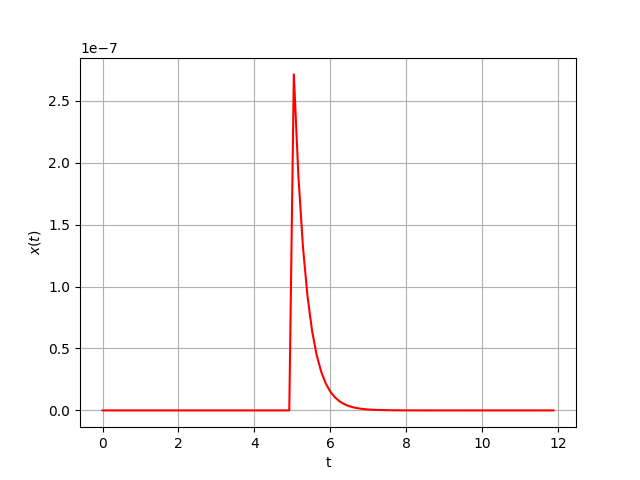
\includegraphics[width=\columnwidth]{figs/x_t.png}
    \caption[short]{Plot of $x\brak{t}$ vs $t$. See \tabref{Table:1}}
    \label{fig:2023.in.37.img1}
\end{figure}

%\end{document}

